% Palli Sahayak: An Open-Source Voice AI System for Multilingual Palliative Care in India
% Target: npj Digital Medicine (Nature portfolio)
% Authors: Ashish Makani, Anurag Agrawal
% Date: February 2026
% Type: Systems/Design Paper with Evaluation Protocol
% Version: v1 — includes Sarvam AI integration (22 Indian language ASR)

\documentclass[11pt,a4paper]{article}

% ============================================================
% PACKAGES
% ============================================================
\usepackage[utf8]{inputenc}
\usepackage[T1]{fontenc}
% Using default Computer Modern (Times fonts not available on this system)
\usepackage[margin=2.5cm]{geometry}
\usepackage{graphicx}
\usepackage{booktabs}
\usepackage{tabularx}
\usepackage{array}
\usepackage{xcolor}
\usepackage{hyperref}
\usepackage{amsmath}
\usepackage{float}
% enumitem not available; using default lists
\usepackage{caption}
\usepackage{subcaption}
\usepackage{setspace}
% Using numeric citation style
\usepackage{url}
\usepackage{tikz}
\usetikzlibrary{shapes.geometric, arrows.meta, positioning, fit, backgrounds, calc}

% ============================================================
% COLORS (Saloni-compliant: colorblind-friendly, concept-matched)
% ============================================================
\definecolor{inputblue}{HTML}{4477AA}      % Input channels
\definecolor{processgreen}{HTML}{228833}   % Processing/RAG
\definecolor{safetyorange}{HTML}{EE6677}   % Safety systems
\definecolor{outputpurple}{HTML}{AA3377}   % Output/delivery
\definecolor{memoryblue}{HTML}{66CCEE}     % Longitudinal memory
\definecolor{neutralgray}{HTML}{BBBBBB}    % Neutral/background
\definecolor{linkblue}{HTML}{0077BB}       % Hyperlinks
\definecolor{sarvamteal}{HTML}{009988}     % Sarvam AI / Indian language

\hypersetup{
    colorlinks=true,
    linkcolor=linkblue,
    citecolor=linkblue,
    urlcolor=linkblue
}

\captionsetup{font=small, labelfont=bf}

% ============================================================
% LINE SPACING
% ============================================================
\onehalfspacing

% ============================================================
% TITLE
% ============================================================
\title{\textbf{Palli Sahayak: An Open-Source Voice AI System for Multilingual Palliative Care in India}}

\author{
Ashish Makani\textsuperscript{1,*} \and
Anurag Agrawal\textsuperscript{1}
}

\date{
\textsuperscript{1}Koita Centre for Digital Health (KCDH-A), Ashoka University, Sonipat, India \\[0.5em]
\textsuperscript{*}Corresponding author: spiff007@gmail.com \\[1em]
\textit{Pre-print --- February 2026}
}

\begin{document}
\maketitle

% ============================================================
% ABSTRACT
% ============================================================
\begin{abstract}
\noindent
Over 10 million Indians require palliative care, yet fewer than 2\% have access to trained providers. India's million-plus Accredited Social Health Activists (ASHA workers) lack palliative care training, and most clinical resources exist only in English despite India's 22 scheduled languages. We present Palli Sahayak, an open-source, voice-first AI helpline that provides around-the-clock palliative care guidance in 22 Indian languages. The system integrates five architectural components: (i)~a hybrid retrieval-augmented generation pipeline combining Microsoft GraphRAG with community-based search, ChromaDB vector retrieval, and a Neo4j knowledge graph, unified through Reciprocal Rank Fusion; (ii)~a multi-provider voice architecture spanning telephone (Bolna.ai), web (Gemini Live API), Indian public switched telephone network (Retell.ai), and Sarvam AI for native Indian language speech recognition across all 22 scheduled languages and text-to-speech synthesis in 11 languages, with automatic failover and a free-tier fallback pipeline; (iii)~a five-pillar clinical safety framework encompassing evidence grading, multilingual emergency detection, medication adherence reminders, response length optimization, and human handoff via SIP-REFER; (iv)~a longitudinal patient context memory system with Fast Healthcare Interoperability Resources (FHIR) R4 interoperability; and (v)~Sarvam AI's Saaras v3 automatic speech recognition engine, purpose-built for Indian languages, providing coverage of all 22 constitutionally scheduled languages---from Hindi and Bengali to Bodo, Dogri, and Santhali---at a cost of approximately \$0.36 per hour. We describe a comprehensive evaluation protocol including retrieval quality benchmarking across search modalities, safety system validation across languages, voice system latency measurement, and a planned clinician rating study with palliative care physicians. Built entirely on free-tier APIs with local-first data storage, the system requires zero infrastructure cost for core deployment. Palli Sahayak is MIT-licensed and positioned as a Digital Public Good. It was demonstrated at the EkStep Voice AI Event in January 2026 with clinicians from the Cipla Foundation.

\vspace{0.5em}
\noindent\textbf{Keywords:} palliative care, voice AI, retrieval-augmented generation, multilingual, India, digital health, FHIR, clinical safety, Sarvam AI, Indian languages
\end{abstract}

% ============================================================
% 1. INTRODUCTION
% ============================================================
\section{Introduction}

\subsection{The Palliative Care Crisis in India}

The World Health Organization estimates that 57 million people globally require palliative care each year, with 78\% residing in low- and middle-income countries (LMICs)\cite{who2020}. India bears a disproportionate share of this burden: more than 10 million patients need palliative care, yet fewer than 2\% have access to trained providers\cite{knaul2018}. The Lancet Commission on Palliative Care and Pain Relief described this disparity as an ``access abyss,'' noting that the poorest nations bear the greatest burden of serious health-related suffering while possessing the fewest resources to address it.

India's community health infrastructure relies on over one million ASHA workers who serve as the primary link between rural communities and the formal healthcare system. Despite their critical role, ASHA workers receive no standardized training in palliative care, leaving them ill-equipped to manage symptoms such as pain, nausea, and breathlessness, or to provide emotional support to patients and families facing serious illness\cite{knaul2018}. The morphine availability crisis compounds this gap: India consumes less than 1\% of global medical opioids despite constituting 17\% of the world's population, largely due to restrictive narcotics regulations\cite{rajagopal2007}.

A further barrier is linguistic. India recognizes 22 scheduled languages, yet clinical palliative care resources---guidelines, training materials, and decision-support tools---exist predominantly in English. The state of Kerala represents a notable exception, having developed a community-based palliative care model that achieves near-universal coverage through local self-government institutions\cite{palat2012, kerala2025}. However, this model depends on trained volunteers and cannot be scaled nationally without technological augmentation.

\subsection{Why Voice-First}

India has 1.2 billion mobile subscribers, yet digital literacy remains low in rural areas where an estimated 30\% of internet users interact primarily through voice\cite{abdm2024}. ASHA workers, many of whom have limited smartphone literacy, are more comfortable speaking than typing. Voice interaction eliminates reading and writing barriers, making health information accessible to populations that text-based systems cannot reach.

Existing health AI systems illustrate this gap. Med-PaLM~2\cite{singhal2024} demonstrated near-expert-level medical question answering, and commercial platforms such as Ada Health and Babylon Health have shown promise in symptom assessment. However, these systems are uniformly text-first and predominantly English-focused. India's national telemedicine service, eSanjeevani, has served over 330 million consultations\cite{sharma2024, esanjeevani2025}, but operates through human teleconsultation without AI augmentation. No existing system combines voice AI, retrieval-augmented generation (RAG), palliative care domain expertise, and comprehensive Indian language support spanning all 22 scheduled languages.

\subsection{Contributions}

We present Palli Sahayak (Hindi: \textit{companion helper}), an open-source voice AI helpline for palliative care in India. The system makes the following contributions:

\begin{enumerate}
    \item The first open-source, voice-first palliative care AI helpline supporting all 22 constitutionally scheduled Indian languages through Sarvam AI's Saaras v3 automatic speech recognition, with text-to-speech synthesis in 11 languages via Sarvam's Bulbul v3 engine.
    \item A hybrid RAG pipeline combining Microsoft GraphRAG\cite{edge2024}, ChromaDB vector search, and Neo4j knowledge graph retrieval with domain-specific entity extraction for palliative care.
    \item A multi-provider voice architecture with automatic failover across five platforms (Bolna.ai, Gemini Live API, Retell.AI, Sarvam AI, and a free-tier fallback pipeline), unified by a common safety wrapper.
    \item A five-pillar clinical safety framework encompassing evidence badges, multilingual emergency detection, medication voice reminders, response length optimization, and human handoff via SIP-REFER.
    \item A longitudinal patient context memory system inspired by MedAgentBench\cite{medagentbench2025}, with FHIR R4 interoperability and temporal reasoning across seven data modalities.
\end{enumerate}

The system is funded by a Grand Challenges India grant from the Biotechnology Industry Research Assistance Council (BIRAC) and the Department of Biotechnology (DBT), with support from the Bill \& Melinda Gates Foundation (India). Clinical partnerships include Max Healthcare (Delhi) and Pallium India (Kerala).

% ============================================================
% 2. RELATED WORK
% ============================================================
\section{Related Work}

\subsection{AI for Palliative Care}

A recent scoping review of 125 studies on artificial intelligence in palliative care found that 86\% were retrospective proof-of-concept investigations, predominantly focused on mortality prediction and natural language processing of clinical notes\cite{nikoloudi2025}. No deployed voice-based system was identified. A separate systematic meta-review of digital health interventions in palliative care identified videoconferencing (17\%), electronic health records (16\%), and telephone (13\%) as the dominant modalities, with no AI-powered voice systems reported\cite{bradford2021}. Reviews of ethical challenges in end-of-life AI applications have highlighted the need for transparent uncertainty communication and safety guardrails\cite{ethicalai2025}, while analyses of foundational gaps have called for external validation and clinical implementation\cite{jpain2025}. Palli Sahayak addresses this implementation gap directly.

\subsection{Voice AI in Healthcare}

Commercial voice AI in healthcare has focused on clinical documentation for providers in high-income settings. Nuance DAX (now Microsoft Dragon Copilot) reduces physician documentation burden through ambient listening\cite{tierney2024}. Suki AI serves over 250 health organizations across 30 specialties in the United States. Hume AI's Empathic Voice Interface detects and responds to emotions in real time, with healthcare deployments in preventive health and mental health. However, all of these systems target English-speaking clinicians rather than patients, and none address palliative care.

In India, telemedicine has achieved remarkable scale through eSanjeevani, which operates across 131,000 facilities\cite{sharma2024}. Yet this platform is human-operated, and a scoping review of telemedicine barriers in India identified technology literacy, trust, and infrastructure gaps as persistent challenges\cite{telemedbarriers2024}. Laranjo et al.'s systematic review of conversational agents in healthcare found the majority were text-based, and none targeted palliative care in LMICs\cite{laranjo2018}. Palli Sahayak is, to our knowledge, the first patient-facing voice AI system for palliative care in Indian languages.

\subsection{Retrieval-Augmented Generation for Clinical Applications}

RAG, introduced by Lewis et al.\cite{lewis2020}, grounds large language model (LLM) responses in retrieved evidence, reducing hallucination. Microsoft GraphRAG\cite{edge2024} extended this paradigm by constructing knowledge graphs from source documents using Leiden community detection, enabling global (corpus-wide), local (entity-focused), and DRIFT (multi-phase reasoning) search. Medical Graph RAG\cite{wu2025} applied graph-based retrieval to clinical safety, while MedRAG demonstrated that knowledge-graph-enhanced retrieval reduces misdiagnosis\cite{medrag2025}. Evaluations on NICE clinical guidelines showed GraphRAG achieving the highest patient-specificity for multi-hop clinical reasoning\cite{medrxiv2025graphrag}. A comprehensive survey of 30 studies on RAG for healthcare confirmed its effectiveness across diagnostic support, electronic health record summarization, and medical question answering\cite{ragsurvey2025}.

Palli Sahayak's distinction lies in its three-way hybrid architecture---GraphRAG, vector search, and knowledge graph---fused through Reciprocal Rank Fusion (RRF), with entity extraction prompts specifically designed for palliative care concepts (symptoms, medications, conditions, treatments, and side effects).

\subsection{Clinical Safety in Medical AI}

Medical hallucination remains a critical concern. A benchmark of 11 foundation models found that 91.8\% of 70 surveyed clinicians had encountered medical hallucinations, with 84.7\% deeming them potentially harmful; chain-of-thought prompting reduced hallucinations in 86.4\% of comparisons\cite{hallucination2025}. A framework for assessing clinical safety of LLM text summaries, based on 12,999 clinician-annotated sentences, reported a 1.47\% hallucination rate\cite{npjsafety2025}. Approaches to automating the GRADE evidence-grading framework have shown promise\cite{gradeauto2025}, and AI-based emergency department triage has consistently achieved area under the curve above 0.80 for high-acuity detection\cite{nejmtriage2024}. Palli Sahayak incorporates evidence grading, hallucination detection, and emergency triage within a unified safety framework designed for voice-first palliative care.

\subsection{Multilingual Healthcare AI for Indian Languages}

The AI4Bharat consortium's IndicVoices dataset provides 12,000 hours of speech across 22 Indian languages from 208 districts\cite{indicvoices2024}, while IndicVoices-R offers 1,704 hours of high-quality text-to-speech data\cite{indicvoicesr2024}. OpenAI's Whisper achieves robust multilingual automatic speech recognition (ASR)\cite{radford2023}. India's Bhashini platform, through a memorandum of understanding with the National Health Authority, is integrating multilingual AI into Ayushman Bharat health platforms. EkStep's Vakyansh provides open-source ASR models for Indic languages.

Sarvam AI, an Indian AI research company, has developed purpose-built models for Indian language processing\cite{sarvam2025}. Their Saaras v3 ASR engine supports all 22 constitutionally scheduled Indian languages---including low-resource languages such as Bodo, Dogri, Kashmiri, Konkani, Maithili, Manipuri, Nepali, Sanskrit, Santhali, and Sindhi---achieving state-of-the-art accuracy on Indian language benchmarks. Their Bulbul v3 text-to-speech engine synthesizes natural speech in 11 Indian languages with over 30 distinct voices, including language-appropriate male and female voices for each supported language. At approximately INR~30 per hour for speech recognition (roughly \$0.36) and INR~30 per 10,000 characters for synthesis, Sarvam's pricing is designed for high-volume, resource-constrained deployments in India.

Palli Sahayak integrates Sarvam AI as a core voice provider alongside Whisper, Deepgram, Edge TTS, and Cartesia, achieving coverage of all 22 scheduled Indian languages for the first time in a healthcare voice AI system.

\subsection{Longitudinal Patient Memory in AI Systems}

MedAgentBench\cite{medagentbench2025} established a FHIR-compliant virtual electronic health record (EHR) environment with 300 physician-written tasks spanning 100 patient profiles. FHIR-Former\cite{fhirformer2025} demonstrated FHIR integration with LLMs for clinical prediction, while LLMonFHIR\cite{llmonfhir2025} enabled patients to query their own health records through conversational interfaces with multilingual support. Stanford's Human-Centered AI group argued that longitudinal datasets address the ``missing context problem'' in healthcare AI\cite{stanfordhai2024}. Palli Sahayak extends this paradigm to voice-first, patient-facing palliative care with cross-modal data aggregation across seven modalities.

% ============================================================
% 3. SYSTEM ARCHITECTURE
% ============================================================
\section{System Architecture}

Palli Sahayak comprises approximately 30,000 lines of Python code organized into ten modules (Table~\ref{tab:components}). The architecture follows a pipeline design in which user input from any channel traverses a unified safety layer before reaching the hybrid RAG engine and response generation (Figure~\ref{fig:architecture}).

\begin{table}[htbp]
\centering
\caption{\textbf{System component inventory.} Each module is independently deployable with defined interfaces. Lines of code (LOC) are approximate and exclude test files.}
\label{tab:components}
\begin{tabular}{@{}llrl@{}}
\toprule
\textbf{Module} & \textbf{Key Files} & \textbf{LOC} & \textbf{Function} \\
\midrule
Core RAG Server & simple\_rag\_server.py & 7,200 & FastAPI server, RAG pipeline, admin UI \\
Safety System & safety\_enhancements.py & 1,500 & Five-pillar safety framework \\
Voice Router & voice\_router.py & 850 & Multi-provider routing and failover \\
Longitudinal Memory & personalization/*.py & 8,500 & Patient context, temporal reasoning, FHIR \\
GraphRAG Wrapper & graphrag\_integration/*.py & 2,500 & Microsoft GraphRAG integration \\
Bolna Integration & bolna\_integration/*.py & 2,000 & Telephone voice AI \\
Sarvam Integration & sarvam\_integration/*.py & 1,400 & Indian language STT/TTS (22 languages) \\
Clinical Validation & clinical\_validation/*.py & 1,800 & Automated clinical checks \\
WhatsApp Bot & whatsapp\_bot.py & 3,000 & Twilio WhatsApp integration \\
Knowledge Graph & knowledge\_graph/*.py & 1,500 & Neo4j entity relationships \\
\midrule
\textbf{Total} & & \textbf{${\sim}$30,250} & \\
\bottomrule
\end{tabular}
\end{table}

% --- FIGURE 1: System Architecture ---
\begin{figure}[htbp]
\centering
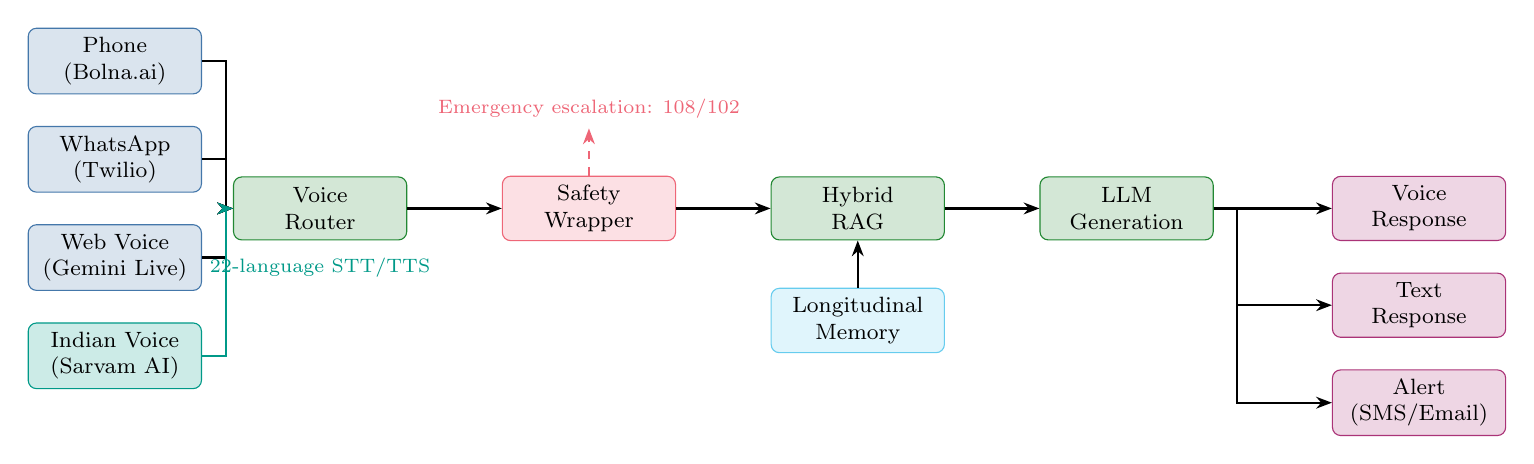
\begin{tikzpicture}[
    node distance=0.8cm and 1.2cm,
    box/.style={rectangle, draw, rounded corners=3pt, minimum width=2.2cm, minimum height=0.8cm, font=\footnotesize, align=center},
    inputbox/.style={box, fill=inputblue!20, draw=inputblue},
    procbox/.style={box, fill=processgreen!20, draw=processgreen},
    safebox/.style={box, fill=safetyorange!20, draw=safetyorange},
    outbox/.style={box, fill=outputpurple!20, draw=outputpurple},
    membox/.style={box, fill=memoryblue!20, draw=memoryblue},
    sarvambox/.style={box, fill=sarvamteal!20, draw=sarvamteal},
    arrow/.style={-{Stealth[length=2mm]}, thick},
]
    % Input channels - directly labeled (no legend per Saloni)
    \node[inputbox] (phone) {Phone\\(Bolna.ai)};
    \node[inputbox, below=0.4cm of phone] (whatsapp) {WhatsApp\\(Twilio)};
    \node[inputbox, below=0.4cm of whatsapp] (web) {Web Voice\\(Gemini Live)};
    \node[sarvambox, below=0.4cm of web] (sarvam) {Indian Voice\\(Sarvam AI)};

    % Voice Router
    \node[procbox, right=1.5cm of $(whatsapp)!0.5!(web)$] (router) {Voice\\Router};

    % Sarvam STT/TTS label
    \node[font=\scriptsize, text=sarvamteal, below=0.1cm of router] {22-language STT/TTS};

    % Safety
    \node[safebox, right=1.2cm of router] (safety) {Safety\\Wrapper};

    % RAG
    \node[procbox, right=1.2cm of safety] (rag) {Hybrid\\RAG};

    % LLM
    \node[procbox, right=1.2cm of rag] (llm) {LLM\\Generation};

    % Memory
    \node[membox, below=0.6cm of rag] (memory) {Longitudinal\\Memory};

    % Outputs - directly labeled
    \node[outbox, right=1.5cm of llm] (voice_out) {Voice\\Response};
    \node[outbox, below=0.4cm of voice_out] (text_out) {Text\\Response};
    \node[outbox, below=0.4cm of text_out] (alert_out) {Alert\\(SMS/Email)};

    % Arrows
    \draw[arrow] (phone.east) -- ++(0.3,0) |- (router.west);
    \draw[arrow] (whatsapp.east) -- ++(0.3,0) |- (router.west);
    \draw[arrow] (web.east) -- ++(0.3,0) |- (router.west);
    \draw[arrow, sarvamteal] (sarvam.east) -- ++(0.3,0) |- (router.west);

    \draw[arrow] (router) -- (safety);
    \draw[arrow] (safety) -- (rag);
    \draw[arrow] (rag) -- (llm);
    \draw[arrow] (memory) -- (rag);

    \draw[arrow] (llm.east) -- ++(0.3,0) |- (voice_out.west);
    \draw[arrow] (llm.east) -- ++(0.3,0) |- (text_out.west);
    \draw[arrow] (llm.east) -- ++(0.3,0) |- (alert_out.west);

    % Safety escalation
    \draw[arrow, safetyorange, dashed] (safety.north) -- ++(0,0.6) node[above, font=\scriptsize, text=safetyorange] {Emergency escalation: 108/102};

\end{tikzpicture}
\caption{\textbf{Palli Sahayak system architecture.} User input from four channels (telephone, WhatsApp, web, and Sarvam AI Indian voice) passes through a voice router and unified safety wrapper before reaching the hybrid RAG pipeline. Sarvam AI provides native Indian language ASR (22 languages) and TTS (11 languages) within the voice router, enabling speech processing for all constitutionally scheduled Indian languages. The longitudinal memory module injects patient context into queries. Outputs are delivered as voice, text, or proactive alerts. Emergency escalation bypasses the RAG pipeline entirely. Components are directly labeled following data visualization best practices; colors encode functional categories (blue: input, green: processing, red-pink: safety, purple: output, cyan: memory, teal: Sarvam AI/Indian language).}
\label{fig:architecture}
\end{figure}

\subsection{Hybrid RAG Pipeline}

The retrieval pipeline queries three backends in parallel and unifies results through Reciprocal Rank Fusion (Figure~\ref{fig:rag}).

\paragraph{Vector search.} Documents are processed into 1,000-character chunks with 200-character overlap and embedded using BAAI/bge-small-en-v1.5 (384 dimensions). ChromaDB stores embeddings locally with cosine similarity retrieval, returning the top five documents per query.

\paragraph{GraphRAG.} Microsoft GraphRAG version 2.7 constructs a knowledge graph from the document corpus through LLM-based entity extraction, followed by Leiden community detection and hierarchical community report generation\cite{edge2024}. Entity extraction uses domain-specific prompts tuned for palliative care concepts: symptoms (pain, nausea, breathlessness), medications (morphine, ondansetron, dexamethasone), conditions (cancer, COPD, heart failure), treatments (radiation, chemotherapy, physiotherapy), and side effects (constipation, sedation, nausea). Four search strategies are available: \textit{global} search synthesizes community reports for corpus-wide queries; \textit{local} search traverses entity neighborhoods for specific queries; \textit{DRIFT} search performs multi-phase reasoning across communities and entities; and \textit{basic} search provides vector similarity as a fallback. An automatic method selector routes queries based on pattern matching (Table~\ref{tab:searchheuristics}).

\begin{table}[htbp]
\centering
\caption{\textbf{GraphRAG search method auto-selection heuristics.} The system classifies incoming queries by pattern and routes them to the most appropriate search strategy.}
\label{tab:searchheuristics}
\begin{tabular}{@{}lll@{}}
\toprule
\textbf{Query Pattern} & \textbf{Method} & \textbf{Rationale} \\
\midrule
Broad or thematic (``guidelines for\ldots'') & Global & Requires corpus-wide synthesis \\
Specific entity (``morphine dosage'') & Local & Entity-focused retrieval \\
Multi-hop (``why is X causing Y'') & DRIFT & Cross-entity reasoning \\
Simple factual (``what is palliative care'') & Basic & Direct vector match sufficient \\
Default or ambiguous & Local & Best general-purpose performance \\
\bottomrule
\end{tabular}
\end{table}

\paragraph{Knowledge graph.} A Neo4j graph database stores medical entities and relationships extracted through LLM-based extraction augmented with regular expression patterns. Five node types (Symptom, Medication, Condition, Treatment, SideEffect) and five relationship types (TREATS, CAUSES, SIDE\_EFFECT\_OF, MANAGES, ALLEVIATES\_WITH) encode clinical knowledge. Natural language queries are translated to Cypher graph queries for traversal.

\paragraph{Fusion.} Results from all three backends are combined using Reciprocal Rank Fusion:
\begin{equation}
\text{RRF}(d) = \sum_{i=1}^{n} \frac{1}{k + \text{rank}_i(d)}
\end{equation}
where $k = 60$ is the standard smoothing constant and $\text{rank}_i(d)$ is the rank of document $d$ in retriever $i$. This approach avoids score normalization across heterogeneous retrieval systems while preserving the relative ordering from each backend.

% --- FIGURE 2: RAG Pipeline ---
\begin{figure}[htbp]
\centering
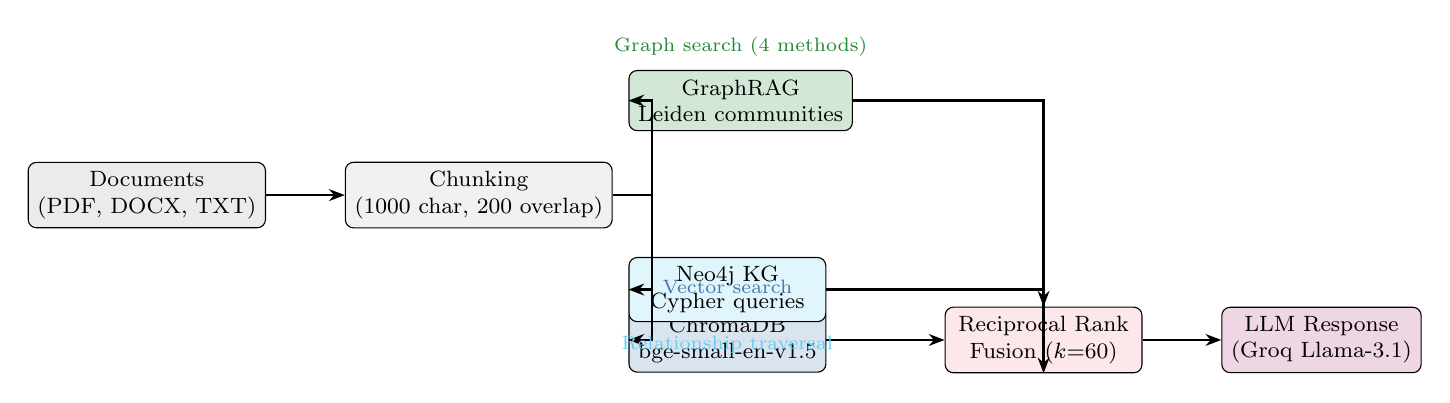
\begin{tikzpicture}[
    node distance=0.6cm and 1.0cm,
    box/.style={rectangle, draw, rounded corners=3pt, minimum width=2.5cm, minimum height=0.7cm, font=\footnotesize, align=center},
    arrow/.style={-{Stealth[length=2mm]}, thick},
]
    % Documents
    \node[box, fill=neutralgray!30] (docs) {Documents\\(PDF, DOCX, TXT)};

    % Chunking
    \node[box, fill=neutralgray!20, right=1.0cm of docs] (chunk) {Chunking\\(1000 char, 200 overlap)};

    % Three paths
    \node[box, fill=inputblue!20, below right=1.0cm and 0.2cm of chunk] (chroma) {ChromaDB\\bge-small-en-v1.5};
    \node[box, fill=processgreen!20, right=0.2cm of chunk, yshift=1.2cm] (graphrag) {GraphRAG\\Leiden communities};
    \node[box, fill=memoryblue!20, right=0.2cm of chunk, yshift=-1.2cm] (neo4j) {Neo4j KG\\Cypher queries};

    % RRF
    \node[box, fill=safetyorange!15, right=1.5cm of chroma] (rrf) {Reciprocal Rank\\Fusion ($k{=}60$)};

    % LLM
    \node[box, fill=outputpurple!20, right=1.0cm of rrf] (llm) {LLM Response\\(Groq Llama-3.1)};

    % Arrows
    \draw[arrow] (docs) -- (chunk);
    \draw[arrow] (chunk.east) -- ++(0.5,0) |- (graphrag.west);
    \draw[arrow] (chunk.east) -- ++(0.5,0) |- (chroma.west);
    \draw[arrow] (chunk.east) -- ++(0.5,0) |- (neo4j.west);
    \draw[arrow] (graphrag.east) -| (rrf.north);
    \draw[arrow] (chroma.east) -- (rrf.west);
    \draw[arrow] (neo4j.east) -| (rrf.south);
    \draw[arrow] (rrf) -- (llm);

    % Direct labels on paths (Saloni: label directly, no legend)
    \node[font=\scriptsize, text=inputblue, above=0.05cm of chroma] {Vector search};
    \node[font=\scriptsize, text=processgreen, above=0.05cm of graphrag] {Graph search (4 methods)};
    \node[font=\scriptsize, text=memoryblue, below=0.05cm of neo4j] {Relationship traversal};

\end{tikzpicture}
\caption{\textbf{Hybrid RAG pipeline.} Documents are chunked and indexed into three parallel retrieval backends: ChromaDB (dense vector search), Microsoft GraphRAG (community-based graph search with four strategies), and Neo4j (relationship traversal via Cypher). Results are fused through Reciprocal Rank Fusion before LLM response generation. Each path is directly labeled with its retrieval modality.}
\label{fig:rag}
\end{figure}

\subsection{Multi-Provider Voice Architecture}

A voice router module dispatches incoming interactions to the most appropriate provider based on channel type (telephone versus web), provider health status, and language requirements (Table~\ref{tab:voiceproviders}). If the primary provider fails, the system cascades through alternatives with automatic failover. The addition of Sarvam AI as a fifth provider dramatically expands Indian language coverage, particularly for the 11 constitutionally scheduled languages that no other commercial voice AI provider currently supports with native ASR.

\begin{table}[htbp]
\centering
\caption{\textbf{Voice provider comparison.} Five providers offer complementary capabilities across channel, language, and cost dimensions. Sarvam AI provides the broadest Indian language coverage with purpose-built ASR (22 languages) and TTS (11 languages). Latency values are approximate first-token-of-speech measurements.}
\label{tab:voiceproviders}
\small
\begin{tabular}{@{}llllll@{}}
\toprule
\textbf{Feature} & \textbf{Bolna.ai} & \textbf{Gemini Live} & \textbf{Retell.AI} & \textbf{Sarvam AI} & \textbf{Fallback} \\
\midrule
Channel & Telephone & Web (WS) & Telephone & Any & Any \\
ASR engine & Deepgram & Native & Deepgram & Saaras v3 & Groq Whisper \\
LLM & GPT-4o-mini & Gemini 2.0 & Custom & Custom & Llama-3.1-8b \\
TTS engine & Cartesia & Native & Cartesia & Bulbul v3 & Edge TTS \\
Latency & ${\sim}$1.5\,s & ${\sim}$0.8\,s & ${\sim}$1.2\,s & ${\sim}$1.0\,s & ${\sim}$2.5\,s \\
ASR languages & 6 & 4 & 4 & \textbf{22} & 5 \\
TTS languages & 6 & 4 & 4 & \textbf{11} & 5 \\
Cost & Per minute & Free & Per minute & INR~30/hr & Free \\
Warm handoff & Via transfer & N/A & SIP-REFER & N/A & N/A \\
RAG integration & Function call & Context inj. & WS LLM & Direct & Direct \\
\bottomrule
\end{tabular}
\end{table}

\paragraph{Bolna.ai.} The primary telephone provider integrates Deepgram Nova-3 for ASR with two-second silence tolerance, GPT-4o-mini for language understanding, and Cartesia Sonic-3 for text-to-speech synthesis via Twilio's public switched telephone network. A custom function call mechanism routes queries to the RAG pipeline through a dedicated \texttt{/api/bolna/query} endpoint, injecting retrieved context into the voice agent's response. Post-call extraction identifies the user's primary concern, emotional state, language used, and urgency level.

\paragraph{Gemini Live API.} For web-based voice interactions, the Gemini Live API provides native bidirectional audio streaming over WebSocket at 16\,kHz input and 24\,kHz output. RAG context is injected through a query classifier that distinguishes information-seeking utterances (routed to the RAG pipeline) from conversational exchanges (handled directly by Gemini).

\paragraph{Retell.AI.} This provider offers SIP-REFER warm handoff capability through Vobiz.ai's Indian PSTN infrastructure with +91 direct inward dialing numbers. When the system determines that a patient requires human clinical attention, SIP-REFER transfers the active call to a physician while preserving the full conversation context and generating a handoff summary.

\paragraph{Sarvam AI.} Sarvam AI serves as the dedicated Indian language voice provider, integrating two purpose-built models for Indian speech processing\cite{sarvam2025}. The Saaras v3 ASR engine supports all 22 constitutionally scheduled Indian languages (Hindi, Bengali, Kannada, Malayalam, Marathi, Odia, Punjabi, Tamil, Telugu, English, Gujarati, Assamese, Bodo, Dogri, Goan Konkani, Kashmiri, Konkani, Maithili, Manipuri, Nepali, Sanskrit, and Sindhi) with three transcription modes: \textit{formal} (standard orthography), \textit{code-mixed} (handling Hindi-English and other code-switching), and \textit{spoken-form} (colloquial transcription). The Bulbul v3 TTS engine synthesizes natural speech in 11 languages with over 30 distinct voices, including gender-appropriate voices per language (for example, Meera and Amol for Hindi, Diya and Arnab for Bengali, Pavithra and Raghav for Kannada). For the 11 STT-only languages without native TTS (Assamese, Bodo, Dogri, Goan Konkani, Kashmiri, Konkani, Maithili, Manipuri, Nepali, Sanskrit, Sindhi), the system falls back to Hindi TTS, which is mutually intelligible for speakers of most North Indian and Indo-Aryan language varieties. The Sarvam integration module also provides real-time WebSocket streaming for both STT and TTS, enabling low-latency voice interactions, and a translation API for cross-language support. Authentication uses Sarvam's API subscription key model. The voice router prioritizes Sarvam for web-based Indian language interactions and as a fallback STT/TTS provider for the pipeline, with Bolna remaining primary for telephone calls.

\paragraph{Fallback pipeline.} When all commercial providers are unavailable, a fully free fallback pipeline chains Groq Whisper (speech-to-text), the RAG pipeline, Groq Llama-3.1-8b-instant (response generation), and Microsoft Edge TTS (text-to-speech synthesis). This pipeline supports five languages (Hindi, English, Bengali, Tamil, Gujarati) at zero API cost.

% --- FIGURE 3: Voice Provider Architecture ---
\begin{figure}[htbp]
\centering
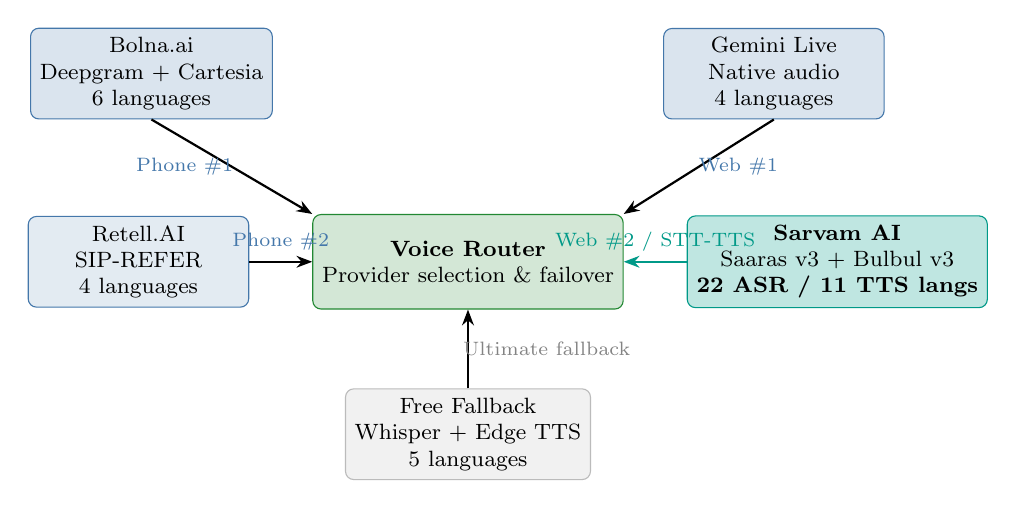
\begin{tikzpicture}[
    node distance=0.5cm and 0.8cm,
    box/.style={rectangle, draw, rounded corners=3pt, minimum width=2.8cm, minimum height=0.7cm, font=\footnotesize, align=center},
    arrow/.style={-{Stealth[length=2mm]}, thick},
]
    % Voice Router (center)
    \node[box, fill=processgreen!20, draw=processgreen, minimum width=3.5cm, minimum height=1.2cm] (router) {\textbf{Voice Router}\\Provider selection \& failover};

    % Providers
    \node[box, fill=inputblue!20, draw=inputblue, above left=1.2cm and 0.5cm of router] (bolna) {Bolna.ai\\Deepgram + Cartesia\\6 languages};
    \node[box, fill=inputblue!20, draw=inputblue, above right=1.2cm and 0.5cm of router] (gemini) {Gemini Live\\Native audio\\4 languages};
    \node[box, fill=inputblue!15, draw=inputblue, left=0.8cm of router] (retell) {Retell.AI\\SIP-REFER\\4 languages};
    \node[box, fill=sarvamteal!25, draw=sarvamteal, right=0.8cm of router, minimum width=3.0cm] (sarvam) {\textbf{Sarvam AI}\\Saaras v3 + Bulbul v3\\\textbf{22 ASR / 11 TTS langs}};
    \node[box, fill=neutralgray!20, draw=neutralgray, below=1.0cm of router] (fallback) {Free Fallback\\Whisper + Edge TTS\\5 languages};

    % Arrows to router
    \draw[arrow] (bolna.south) -- (router.north west);
    \draw[arrow] (gemini.south) -- (router.north east);
    \draw[arrow] (retell.east) -- (router.west);
    \draw[arrow, sarvamteal, thick] (sarvam.west) -- (router.east);
    \draw[arrow] (fallback.north) -- (router.south);

    % Priority labels
    \node[font=\scriptsize, text=inputblue] at ($(bolna.south)!0.5!(router.north west)+(-0.6,0)$) {Phone \#1};
    \node[font=\scriptsize, text=inputblue] at ($(gemini.south)!0.5!(router.north east)+(0.5,0)$) {Web \#1};
    \node[font=\scriptsize, text=inputblue] at ($(retell.east)!0.5!(router.west)+(0,0.25)$) {Phone \#2};
    \node[font=\scriptsize, text=sarvamteal] at ($(sarvam.west)!0.5!(router.east)+(0,0.25)$) {Web \#2 / STT-TTS};
    \node[font=\scriptsize, text=neutralgray!70!black] at ($(fallback.north)!0.5!(router.south)+(1.0,0)$) {Ultimate fallback};

\end{tikzpicture}
\caption{\textbf{Multi-provider voice architecture with failover.} The voice router selects providers based on channel type (phone vs.\ web), language requirements, and provider health. Bolna.ai is primary for telephone; Gemini Live is primary for web. Sarvam AI provides the broadest Indian language coverage (22~ASR, 11~TTS) and serves as the preferred STT/TTS engine for the fallback pipeline. Retell.AI provides SIP-REFER warm handoff for clinical escalation. Provider priority labels indicate the routing order per channel.}
\label{fig:voicearch}
\end{figure}

\subsection{Clinical Safety Framework}

All user interactions pass through a five-pillar safety framework before and after response generation (Figure~\ref{fig:safety}).

% --- FIGURE 4: Safety Pipeline ---
\begin{figure}[htbp]
\centering
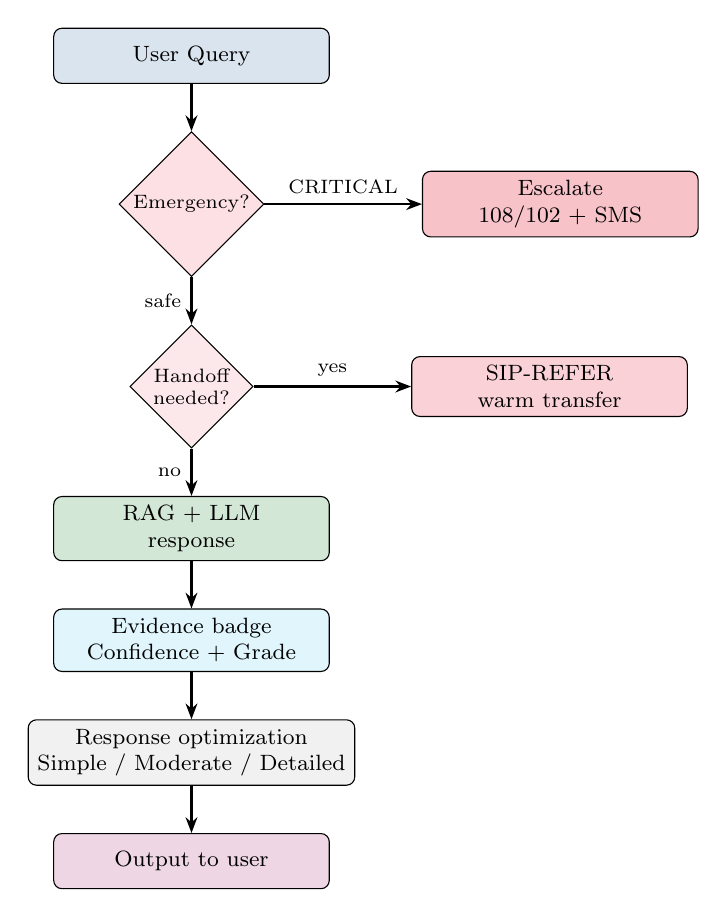
\begin{tikzpicture}[
    node distance=0.7cm,
    box/.style={rectangle, draw, rounded corners=3pt, minimum width=3.5cm, minimum height=0.7cm, font=\footnotesize, align=center},
    decision/.style={diamond, draw, minimum width=1.5cm, minimum height=0.7cm, font=\scriptsize, align=center, inner sep=1pt},
    arrow/.style={-{Stealth[length=2mm]}, thick},
]
    \node[box, fill=inputblue!20] (input) {User Query};
    \node[decision, fill=safetyorange!20, below=0.6cm of input] (emerg) {Emergency?};
    \node[box, fill=safetyorange!40, right=2.0cm of emerg] (escalate) {Escalate\\108/102 + SMS};
    \node[decision, fill=safetyorange!15, below=0.6cm of emerg] (handoff) {Handoff\\needed?};
    \node[box, fill=safetyorange!30, right=2.0cm of handoff] (siprefer) {SIP-REFER\\warm transfer};
    \node[box, fill=processgreen!20, below=0.6cm of handoff] (rag) {RAG + LLM\\response};
    \node[box, fill=memoryblue!20, below=0.6cm of rag] (badge) {Evidence badge\\Confidence + Grade};
    \node[box, fill=neutralgray!20, below=0.6cm of badge] (optimize) {Response optimization\\Simple / Moderate / Detailed};
    \node[box, fill=outputpurple!20, below=0.6cm of optimize] (output) {Output to user};

    \draw[arrow] (input) -- (emerg);
    \draw[arrow] (emerg) -- node[above, font=\scriptsize] {CRITICAL} (escalate);
    \draw[arrow] (emerg) -- node[left, font=\scriptsize] {safe} (handoff);
    \draw[arrow] (handoff) -- node[above, font=\scriptsize] {yes} (siprefer);
    \draw[arrow] (handoff) -- node[left, font=\scriptsize] {no} (rag);
    \draw[arrow] (rag) -- (badge);
    \draw[arrow] (badge) -- (optimize);
    \draw[arrow] (optimize) -- (output);

\end{tikzpicture}
\caption{\textbf{Five-pillar clinical safety pipeline.} Every query passes through sequential safety checks: (1)~emergency detection with immediate escalation to India's 108/102 emergency services, (2)~human handoff assessment with SIP-REFER warm transfer, (3)~RAG-grounded response generation, (4)~evidence badge assignment with confidence scoring and literature grade, and (5)~response length optimization adapted to user comprehension level. Each voice provider, including Sarvam AI, passes through the same unified safety wrapper via a provider-specific safety integration class. Annotations indicate the decision outcome at each stage.}
\label{fig:safety}
\end{figure}

\paragraph{Pillar 1: Evidence badges.} Each response receives a confidence score (0--100\%) and an evidence grade (A through E) mapped to the Oxford Centre for Evidence-Based Medicine levels. Confidence is computed as $1.0 - (d_{\text{vec}} / 2.0)$, where $d_{\text{vec}}$ is the cosine distance to the nearest retrieved document, scaled to a percentage. Source quality is assessed through pattern matching: documents from WHO, NICE, or ASCO guidelines receive high quality scores; blog posts and unverified forum content receive low scores. Grade~A corresponds to systematic reviews and randomized controlled trials, Grade~B to controlled studies, Grade~C to observational studies, Grade~D to expert opinion, and Grade~E triggers an explicit ``please consult your physician'' advisory.

\paragraph{Pillar 2: Emergency detection.} The system maintains keyword-based emergency detection patterns in five languages (English, Hindi, Bengali, Tamil, Gujarati) across three severity levels. CRITICAL triggers---such as ``can't breathe'' (Hindi: \textit{saans nahin aa rahi}), ``unconscious'' (Hindi: \textit{behosh}), or ``heart attack'' (Hindi: \textit{dil ka daura})---cause immediate escalation: the system provides India's emergency numbers (108 for ambulance, 102 for referral transport), sends an SMS to the registered caregiver, and initiates human handoff. HIGH triggers notify caregivers; MEDIUM triggers advise consultation. Sarvam AI's 22-language ASR enables emergency keyword detection to be extended to additional Indian languages as keyword dictionaries are developed.

\paragraph{Pillar 3: Medication voice reminders.} The system places automated outbound telephone calls at scheduled medication times, using language-specific voice templates. Patients confirm medication intake through dual-tone multi-frequency (DTMF) keypress (press~1) or voice confirmation (``yes'' or equivalent in the patient's language). Up to three retry attempts are made for unanswered calls. Adherence rates are tracked as the ratio of confirmed to total scheduled reminders.

\paragraph{Pillar 4: Response length optimization.} Responses are adapted to three comprehension levels. SIMPLE mode limits output to 500 characters, four sentences, and eighth-grade vocabulary. MODERATE mode permits 1,000 characters with medical terms explained in parentheses. DETAILED mode allows 2,000 characters with technical terminology and source citations. The system auto-detects the appropriate level from the user's message length, vocabulary complexity, and question type. For voice output, responses are further constrained to approximately 130 words (30 seconds of speech) with markdown formatting stripped.

\paragraph{Pillar 5: Human handoff.} When any of seven conditions are met---emergency detection, user request, AI uncertainty, complex clinical case, medication dosage query, emotional distress, or repeated identical questions---the system initiates warm transfer. On Retell.AI, this uses the SIP-REFER protocol to transfer the active telephone call to a clinician while preserving conversation context. A unique request identifier is generated for tracking, and a summary is sent to the care team.

\subsection{Longitudinal Patient Context Memory}

Inspired by the MedAgentBench framework\cite{medagentbench2025}, the longitudinal memory system maintains patient records spanning one to five years through a core data primitive: the \texttt{TimestampedObservation}. Each observation captures an event at a point in time, tagged with its source modality (one of seven: voice call, WhatsApp, uploaded document, caregiver report, clinical entry, patient-reported, or FHIR import), reporter identity (patient, caregiver, provider, or system), and clinical category (symptom, medication, vital sign, functional status, or emotional state). Specialized observation types include \texttt{SymptomObservation} (with location, duration, and aggravating or relieving factors), \texttt{MedicationEvent} (started, stopped, dose changed, taken, missed, or side effect reported), and \texttt{VitalSignObservation} (with normal range validation).

A temporal reasoning module analyzes observation sequences to detect trends---improving, stable, worsening, or fluctuating---using linear regression with $R^2$ confidence. It identifies diurnal and weekly patterns, computes severity change rates per week, and analyzes medication effectiveness by correlating medication events with symptom trajectories while accounting for response lag.

A cross-modal aggregation module unifies observations from all seven data sources, applying quality-based weighting (clinical entries weighted highest, self-reports weighted lowest) and resolving conflicts when sources disagree. The aggregated patient context is injected into RAG queries through a context injection module that generates temporal summaries (``pain has worsened from moderate to severe over the past three days; morphine prescribed three days ago shows 60\% symptom improvement'').

For interoperability with hospital electronic health record systems, a FHIR R4 adapter exports longitudinal records as FHIR Bundles containing Patient, Observation, MedicationStatement, Condition, and CareTeam resources. Standard code systems---SNOMED-CT for clinical terminology, LOINC for laboratory and vital signs, ICD-10 for diagnoses, and RxNorm for medications---ensure semantic interoperability. Import is supported bidirectionally.

A proactive alert management module monitors observations against configurable rules (symptom severity thresholds, medication adherence falling below a specified percentage, loss of contact for a specified number of days) and routes multi-channel notifications (WhatsApp, email, dashboard) to appropriate care team members with priority-based escalation.

% ============================================================
% 4. CLINICAL VALIDATION FRAMEWORK
% ============================================================
\section{Clinical Validation Framework}

\subsection{Automated Validation Pipeline}

Every generated response passes through five automated validation layers. First, \textit{medical entity verification} matches extracted entities against SNOMED-CT codes to confirm that referenced symptoms, medications, and conditions correspond to recognized clinical concepts. Second, \textit{dosage range validation} checks any mentioned dosage against a database of 150 or more medications with established safe ranges (for example, morphine oral: 2.5--200\,mg per dose; paracetamol: maximum 4,000\,mg per day; fentanyl transdermal: 12--100\,$\mu$g per hour). Third, \textit{contraindication detection} flags known drug-drug and drug-disease interactions. Fourth, \textit{hallucination detection} verifies that all clinical claims in the response are grounded in the retrieved source documents. Fifth, \textit{evidence grading} assesses source quality against established clinical guidelines from the World Health Organization, Max Healthcare palliative care protocols, and Pallium India morphine guidelines.

\subsection{Expert Sampling System}

A configurable sampling mechanism selects a proportion of queries (default: 5\%) for expert clinical review, with priority sampling for responses flagged by the automated pipeline, low-confidence responses, and queries adjacent to emergency situations. Clinician reviewers score sampled responses on three dimensions: accuracy (0--10), completeness (0--10), and safety (0--10). Tracked aggregate metrics include validation confidence (mean automated confidence score), hallucination rate (proportion of responses flagged for ungrounded claims), expert agreement (concordance between automated and expert assessments), and citation rate (proportion of responses with source attribution).

\subsection{Clinical Test Scenarios}

Four representative clinical scenarios have been implemented as automated test cases to validate system behavior across realistic palliative care situations (Table~\ref{tab:scenarios}).

\begin{table}[htbp]
\centering
\caption{\textbf{Clinical test scenarios.} Each scenario represents a realistic palliative care situation with specific medications, languages, and evaluation focus areas. These serve as regression tests and form the basis for the planned clinician evaluation.}
\label{tab:scenarios}
\small
\begin{tabular}{@{}p{1.5cm}p{2.5cm}p{2.2cm}p{3.5cm}p{3.0cm}@{}}
\toprule
\textbf{Scenario} & \textbf{Patient} & \textbf{Condition} & \textbf{Key Medications} & \textbf{Test Focus} \\
\midrule
Oncology & Mrs.\ Lakshmi Devi, 68F & Stage III breast cancer, AC-T cycle 3/6 & Ondansetron 8\,mg TDS, Dexamethasone 4\,mg BD, Morphine SR 10\,mg BD, Loperamide PRN & Medication reminders, priority scheduling, Hindi voice \\[0.3em]
COPD & Mr.\ Ramesh Patel, 72M & GOLD Stage III COPD & Tiotropium 18\,$\mu$g daily, Salmeterol+Fluticasone 50/500\,$\mu$g BD, Albuterol PRN & Multi-inhalant adherence, device instructions, Gujarati voice \\[0.3em]
Emergency & Same COPD patient & Acute breathlessness & --- & Emergency detection in Gujarati, SIP-REFER handoff, caregiver SMS \\[0.3em]
Evidence & Generic query & Pain management & Morphine & Evidence badge generation with WHO, Max Healthcare, Pallium India citations \\
\bottomrule
\end{tabular}
\end{table}

% ============================================================
% 5. IMPLEMENTATION
% ============================================================
\section{Implementation}

\subsection{Technology Stack}

Palli Sahayak is implemented in Python 3.10 or later, using FastAPI for the REST API and WebSocket server and Gradio for the web-based administration interface. Table~\ref{tab:techstack} summarizes the principal dependencies across system layers.

\begin{table}[htbp]
\centering
\caption{\textbf{Technology stack.} The system is built on open-source and free-tier components. Sarvam AI provides the broadest Indian language coverage for both ASR and TTS. No proprietary database or GPU infrastructure is required for core deployment.}
\label{tab:techstack}
\begin{tabular}{@{}llll@{}}
\toprule
\textbf{Layer} & \textbf{Technology} & \textbf{Version} & \textbf{Role} \\
\midrule
Application server & FastAPI & $\geq$0.104 & REST API, WebSocket \\
Administration UI & Gradio & $\geq$4.7 & Web-based management \\
Vector database & ChromaDB & $\geq$0.4.18 & Dense retrieval \\
Graph database & Neo4j & $\geq$5.14 & Knowledge graph \\
Graph RAG & Microsoft GraphRAG & $\geq$2.7 & Community-based retrieval \\
Embeddings & BAAI/bge-small-en-v1.5 & --- & 384-dim sentence embeddings \\
LLM & Groq (Llama-3.1-8b) & --- & Text generation (free tier) \\
ASR (global) & Groq Whisper & large-v3 & Speech-to-text (free tier) \\
ASR (Indian) & Sarvam Saaras v3 & --- & 22 Indian language STT \\
TTS (global) & Edge TTS & $\geq$6.1 & Speech synthesis (free) \\
TTS (Indian) & Sarvam Bulbul v3 & --- & 11 Indian language, 30+ voices \\
Telephony (primary) & Bolna.ai + Twilio & --- & PSTN voice calls \\
Web voice & Gemini Live API & 2.0 Flash & Audio streaming \\
Telephony (India) & Retell.AI + Vobiz.ai & --- & Indian phone numbers \\
Translation & Sarvam Translate & --- & Cross-language support \\
\bottomrule
\end{tabular}
\end{table}

\subsection{Multilingual Support}

The integration of Sarvam AI's Saaras v3 ASR engine provides speech recognition coverage for all 22 constitutionally scheduled Indian languages, a transformative expansion from the 8-language coverage available through Whisper and Deepgram alone. For text-to-speech synthesis, Sarvam's Bulbul v3 engine supports 11 Indian languages with over 30 natural-sounding voices, including gender-appropriate options for each language (Table~\ref{tab:languages}). For the 11 additional ASR-supported languages without native Sarvam TTS (Assamese, Bodo, Dogri, Goan Konkani, Kashmiri, Konkani, Maithili, Manipuri, Nepali, Sanskrit, and Sindhi), the system falls back to Hindi TTS, leveraging the mutual intelligibility between Hindi and many North Indian languages.

\begin{table}[htbp]
\centering
\caption{\textbf{Language coverage matrix.} The system supports all 22 constitutionally scheduled Indian languages for ASR through Sarvam AI's Saaras v3, with TTS in 11 languages via Bulbul v3. Additional ASR engines (Whisper, Deepgram) and TTS engines (Edge TTS, Cartesia) provide redundant coverage for high-resource languages. Emergency keyword detection is available in five languages, with expansion planned.}
\label{tab:languages}
\small
\begin{tabular}{@{}llp{4.5cm}p{3.5cm}lp{1.5cm}@{}}
\toprule
\textbf{Language} & \textbf{ISO} & \textbf{ASR Engines} & \textbf{TTS Engines} & \textbf{Emergency} & \textbf{Voices} \\
\midrule
Hindi & hi-IN & Sarvam, Whisper, Deepgram & Sarvam, Edge, Cartesia & Full & Meera, Amol \\
English (India) & en-IN & Sarvam, Whisper, Deepgram & Sarvam, Edge, Cartesia & Full & Sita, Neel \\
Bengali & bn-IN & Sarvam, Whisper & Sarvam, Edge & Full & Diya, Arnab \\
Tamil & ta-IN & Sarvam, Whisper, Deepgram & Sarvam, Edge, Cartesia & Full & Thara, Aravind \\
Gujarati & gu-IN & Sarvam, Whisper & Sarvam, Edge & Full & Riddhi, Chirag \\
Marathi & mr-IN & Sarvam, Whisper, Deepgram & Sarvam, Cartesia & Partial & Ananya, Advait \\
Telugu & te-IN & Sarvam & Sarvam & --- & Lakshmi, Karthik \\
Kannada & kn-IN & Sarvam & Sarvam & --- & Pavithra, Raghav \\
Malayalam & ml-IN & Sarvam, Deepgram & Sarvam & --- & Ammu, Arjun \\
Odia & od-IN & Sarvam & Sarvam & --- & Shruti, Manash \\
Punjabi & pa-IN & Sarvam, Deepgram & Sarvam & --- & Divya, Gurpreet \\
\midrule
\multicolumn{6}{@{}l}{\textit{Additional ASR-only languages (Sarvam Saaras v3, TTS falls back to Hindi):}} \\
\midrule
Assamese & as-IN & Sarvam & Hindi fallback & --- & --- \\
Bodo & brx-IN & Sarvam & Hindi fallback & --- & --- \\
Dogri & doi-IN & Sarvam & Hindi fallback & --- & --- \\
Goan Konkani & gom-IN & Sarvam & Hindi fallback & --- & --- \\
Kashmiri & ks-IN & Sarvam & Hindi fallback & --- & --- \\
Konkani & kok-IN & Sarvam & Hindi fallback & --- & --- \\
Maithili & mai-IN & Sarvam & Hindi fallback & --- & --- \\
Manipuri & mni-IN & Sarvam & Hindi fallback & --- & --- \\
Nepali & ne-IN & Sarvam & Hindi fallback & --- & --- \\
Sanskrit & sa-IN & Sarvam & Hindi fallback & --- & --- \\
Sindhi & sd-IN & Sarvam & Hindi fallback & --- & --- \\
\bottomrule
\end{tabular}
\end{table}

The multi-engine architecture provides redundancy for high-resource languages while Sarvam AI provides exclusive coverage for low-resource languages. Hindi and English receive the broadest provider coverage (three ASR engines, three TTS engines, five voice providers). The voice router selects the optimal ASR and TTS engine for each interaction based on language, latency requirements, and provider availability.

\subsection{Zero-Cost Deployment}

A deliberate design goal was to enable deployment with zero infrastructure cost for the core system. The LLM (Groq Llama-3.1-8b-instant) and speech-to-text (Groq Whisper large-v3) operate on Groq's free tier. Text-to-speech uses Microsoft Edge TTS, which requires no API key. Sarvam AI provides INR~1,000 (approximately \$12) in free credits upon signup, sufficient for approximately 33 hours of speech recognition or 333,000 characters of speech synthesis. ChromaDB provides local vector storage without a database server. Sentence embeddings run on CPU without GPU requirements. All patient data is stored locally in JSON files, eliminating cloud storage costs and keeping health data within the deployment environment. The system runs on a single machine and is distributed under the MIT license.

% ============================================================
% 6. EVALUATION PROTOCOL
% ============================================================
\section{Evaluation Protocol}

We describe the methodology for a comprehensive evaluation across four domains. This section presents the evaluation design; results will be reported in a subsequent publication upon completion of the prospective study.

\subsection{Retrieval Quality}

\paragraph{Benchmark construction.} A palliative care question-answering benchmark of 100 items is being constructed from three source guidelines: the WHO Cancer Pain Relief guidelines (2024 edition), the Pallium India Clinical Handbook, and Max Healthcare Palliative Care Protocols. Gold-standard answers will be verified by two palliative care physicians. Questions span five categories: pain management (30\%), symptom control (25\%), medication queries (20\%), emotional support (15\%), and caregiver guidance (10\%).

\paragraph{Metrics.} Retrieval quality will be assessed using Recall@$K$ (for $K \in \{1, 3, 5, 10\}$), Mean Reciprocal Rank (MRR), and Normalized Discounted Cumulative Gain at rank~10 (NDCG@10).

\paragraph{Ablation design.} To quantify the contribution of each retrieval backend, we plan a four-condition ablation study: (A)~ChromaDB vector search only, (B)~GraphRAG only with automatic method selection, (C)~Neo4j knowledge graph only, and (D)~the full hybrid pipeline with RRF fusion. We hypothesize that condition~D will outperform all individual conditions.

\subsection{Safety System Validation}

\paragraph{Emergency detection.} A test set of at least 200 utterances (100 emergency, at least 100 benign) will be constructed across five languages (40 utterances per language, evenly split between emergency and benign categories). Precision, recall, and F1 score will be computed per severity level per language. Adversarial cases---such as past-tense references (``my mother had a heart attack last year'')---will be included to assess false positive rates.

\paragraph{Evidence badge calibration.} One hundred query-response pairs will be assigned expert confidence ratings by two palliative care physicians (ground truth). System-generated confidence scores will be compared using Expected Calibration Error (ECE) and reliability diagrams.

\paragraph{Hallucination detection.} Fifty system responses will be annotated by a clinical expert for grounded claims, unsupported claims, and fabricated information. Detection accuracy, false positive rate, and false negative rate will be reported.

\subsection{Voice System Performance}

\paragraph{End-to-end latency.} Timestamps will be recorded at four pipeline stages: ASR completion, RAG query return, LLM generation completion, and TTS synthesis start. The interval from user speech end to agent speech start will be reported as $p_{50}$, $p_{95}$, and $p_{99}$ latency for each of the five voice providers over 100 test calls per provider.

\paragraph{ASR accuracy.} A test set of 50 palliative care utterances per language will be manually transcribed by native speakers. For the 11 languages with full TTS support via Sarvam, this yields 550 utterances. Word Error Rate (WER) and Character Error Rate (CER) will be computed for each ASR engine where available. For Sarvam's Saaras v3, the three transcription modes (formal, code-mixed, spoken-form) will be evaluated independently.

\paragraph{Failover reliability.} Provider failures (API timeout, HTTP 500 errors, rate limiting) will be simulated programmatically. Failover latency and success rate will be measured over 100 simulated failures per provider.

\paragraph{Sarvam AI-specific evaluation.} For the 11 low-resource languages supported exclusively by Sarvam Saaras v3, a targeted ASR evaluation will use 20 palliative care utterances per language (220 total), recorded by native speakers. WER will be compared against the Whisper large-v3 baseline for languages where Whisper coverage exists (Hindi, Bengali, Tamil, Gujarati, Marathi) to quantify any accuracy differential.

\subsection{Clinical Appropriateness Study}

Fifty queries spanning common palliative care topics will be submitted to the system. At least two palliative care physicians from clinical partner institutions (Max Healthcare and Pallium India) will independently rate each response on a five-point Likert scale across five dimensions: accuracy (medical correctness), safety (absence of harmful advice), empathy (appropriate tone for palliative care), actionability (practical usefulness for an ASHA worker or caregiver), and completeness (coverage of relevant information). Inter-rater reliability will be assessed using Cohen's kappa. Table~\ref{tab:evalprotocol} summarizes the evaluation protocol.

\begin{table}[htbp]
\centering
\caption{\textbf{Evaluation protocol summary.} Ten experiments span four domains. Sample sizes, metrics, and rater requirements are specified for each experiment. Automated experiments require no human raters; clinical experiments involve palliative care physicians from partner institutions.}
\label{tab:evalprotocol}
\small
\begin{tabular}{@{}p{2.8cm}lp{2.5cm}p{3.0cm}l@{}}
\toprule
\textbf{Experiment} & \textbf{Domain} & \textbf{Sample Size} & \textbf{Primary Metrics} & \textbf{Raters} \\
\midrule
Retrieval quality & RAG & 100 Q\&A pairs & Recall@$K$, MRR, NDCG & Automated \\
Retrieval ablation & RAG & 100 Q\&A pairs & Recall@$K$, MRR, NDCG & Automated \\
Emergency detection & Safety & 200+ utterances & Precision, Recall, F1 & Automated \\
Evidence calibration & Safety & 100 pairs & ECE, reliability diagram & 2 clinicians \\
Hallucination detection & Safety & 50 responses & Accuracy, FPR, FNR & 1 expert \\
Voice latency & Voice & 500 calls (5$\times$100) & $p_{50}$/$p_{95}$/$p_{99}$ & Automated \\
ASR accuracy & Voice & 550 utterances & WER, CER & Native speakers \\
Sarvam low-resource ASR & Voice & 220 utterances & WER & Native speakers \\
Failover reliability & Voice & 500 failures (5$\times$100) & Time, success rate & Automated \\
Clinical appropriateness & Clinical & 50 queries & Likert (1--5), $\kappa$ & 2+ physicians \\
\bottomrule
\end{tabular}
\end{table}

% ============================================================
% 7. REAL-WORLD DEPLOYMENT
% ============================================================
\section{Deployment and Demonstration}

Palli Sahayak was demonstrated at the EkStep Voice AI Event on January 28, 2026, at The Ritz-Carlton, Bengaluru, attended by representatives from healthcare organizations, government agencies, and technology companies. A live demonstration was conducted in Marathi with physicians from the Cipla Foundation (Dr.\ Sachin and Dr.\ Prakash), who interacted with the system using clinical vignettes representing common palliative care consultations. The demonstration included voice-based medical queries, evidence badge display, emergency detection, and safety features.

The system operates under a Grand Challenges India grant awarded in November 2024 by BIRAC-DBT with support from the Bill \& Melinda Gates Foundation (India). The principal investigator is Dr.\ Anurag Agrawal (Koita Centre for Digital Health, Ashoka University); the co-investigator and system architect is Ashish Makani (Koita Centre for Digital Health, Ashoka University). Clinical partnerships have been established with Max Healthcare (Delhi) for oncology and palliative care, and Pallium India (Kerala) for community-based palliative care expertise. These partnerships will provide the clinical sites and physician evaluators for the prospective evaluation described in Section~6.

The system source code, comprising approximately 30,000 lines of Python, is publicly available under the MIT license at \url{https://github.com/inventcures/rag_gci}. Documentation, including architecture specifications, API references, and deployment guides, is maintained alongside the code. The system is positioned as a Digital Public Good, aligning with United Nations Sustainable Development Goals~3 (Good Health and Well-being) and~10 (Reduced Inequalities).

% ============================================================
% 8. DISCUSSION
% ============================================================
\section{Discussion}

\subsection{Limitations}

We acknowledge several important limitations. First, and most significantly, this paper describes a system architecture and evaluation protocol; \textit{no prospective clinical outcomes data are reported}. The clinical test scenarios use synthetic patient data, and the system has not been deployed with actual patients. Institutional review board approval and patient consent processes will be required before any prospective evaluation.

Second, the emergency detection system relies on keyword pattern matching rather than contextual natural language understanding. This approach is computationally efficient and language-extensible but susceptible to false positives from past-tense or hypothetical references (for example, ``my mother had a heart attack last year'' would trigger a CRITICAL alert). Future iterations should incorporate contextual intent classification. While Sarvam AI's 22-language ASR enables transcription of emergency utterances in all scheduled languages, emergency keyword dictionaries currently exist for only five languages.

Third, evidence badge confidence scores are computed through heuristic combination of vector distance and source quality pattern matching rather than through a learned calibration model. The relationship between system-assigned confidence and true response accuracy has not been empirically validated.

Fourth, while Sarvam AI's Bulbul v3 provides native TTS in 11 Indian languages---a substantial improvement over the 5-language coverage available through Edge TTS alone---11 ASR-supported languages still fall back to Hindi TTS. This includes languages from diverse language families (Kashmiri, Manipuri, Bodo) for which Hindi may not be readily intelligible. Expanding native TTS coverage to all 22 languages remains a priority.

Fifth, retrieval quality is bounded by the document corpus. The system cannot provide accurate guidance on topics absent from its knowledge base, and corpus comprehensiveness has not been systematically audited against palliative care curricula.

Sixth, the free-tier API constraints that enable zero-cost deployment also impose rate limits. Groq's free tier permits approximately 14,400 tokens per day, which is insufficient for production-scale deployment. Sarvam's free credits (INR~1,000) support approximately 33 hours of ASR, sufficient for initial pilot testing but not sustained operation. Scaling would require paid API access or on-device model deployment.

Seventh, no formal user study has been conducted with ASHA workers, patients, or caregivers. Usability, trust, comprehension, and clinical workflow integration remain unvalidated.

Eighth, the longitudinal patient context memory system, including the FHIR adapter and temporal reasoning module, has been implemented and unit-tested but not validated against real patient trajectories spanning multiple months.

Ninth, while the system handles Hindi-English code-switching (``Hinglish'') through Sarvam's code-mixed transcription mode, it does not robustly manage arbitrary code-switching between other language pairs within single utterances.

\subsection{Future Work}

Near-term priorities include a prospective pilot study with ASHA workers at Max Healthcare and Pallium India clinical sites, an evaluation of retrieval quality and clinical appropriateness using the protocol described in Section~6, and integration with India's Ayushman Bharat Health Account (ABHA) for national health identity linkage. Medium-term goals include a randomized controlled trial comparing ASHA workers using Palli Sahayak with standard-of-care support, deployment of quantized on-device language models (such as Llama~3 at 4-bit precision) for fully offline operation in areas without internet connectivity, active learning from clinician feedback to iteratively improve retrieval quality, expansion of emergency keyword dictionaries to all 22 Sarvam-supported languages, and extension to regional dialects beyond standard language variants. Longer-term, integration with India's 108 emergency medical service for automated dispatch could reduce time to emergency response for critical palliative care situations. As Sarvam AI expands Bulbul v3 TTS coverage to additional languages, the system will automatically gain native synthesis capabilities for those languages without architectural changes.

% ============================================================
% 9. ETHICAL CONSIDERATIONS
% ============================================================
\section{Ethical Considerations}

\subsection{Sensitivity of Palliative Care}

Palliative care interactions involve patients and families navigating serious illness, end-of-life decisions, and profound emotional vulnerability. Cultural and religious beliefs deeply influence attitudes toward death, pain management, and care goals across India's diverse communities. The system is designed with explicit constraints to respect this sensitivity: it never overrides clinical judgment, always advises physician consultation when evidence is uncertain (Grade~D or E), avoids providing specific medication dosages (deferring to the treating physician), and uses compassionate, culturally appropriate language. Nevertheless, the risk of over-reliance by ASHA workers on AI-generated guidance warrants careful monitoring during any prospective deployment. Informed consent processes for vulnerable patient populations must account for power dynamics, health literacy, and the patient's capacity to understand the nature of AI-mediated information.

\subsection{Data Privacy}

The system follows a local-first data architecture: all patient data, including longitudinal records, medication schedules, and conversation histories, are stored on the deployment machine's local filesystem in JSON format. No personal health information is transmitted to third-party LLM APIs; queries to Groq or OpenAI contain only retrieved document context, not patient identifiers. Voice recordings are not persistently stored. Audio sent to Sarvam AI for speech recognition contains only the speech signal without patient identifiers; Sarvam's servers are hosted in India, ensuring data residency within national borders. FHIR export is an opt-in function requiring explicit patient or caregiver consent. The system's data handling practices are designed to align with India's Digital Personal Data Protection Act (DPDP Act, 2023), though formal compliance certification has not been obtained and will be pursued as part of the prospective deployment.

\subsection{Bias and Equity}

Language bias is an inherent limitation: ASR and TTS quality is higher for well-resourced languages (Hindi, English) than for under-resourced languages (Bodo, Manipuri, Sindhi), reflecting disparities in available training data. Sarvam AI's purpose-built Indian language models mitigate this gap substantially---supporting ASR for all 22 scheduled languages where global models like Whisper cover only 5--6---but accuracy differentials across languages have not been quantified. The system requires internet connectivity, which disadvantages rural areas with limited infrastructure. Currently available TTS voices are predominantly female across most Sarvam-supported languages, potentially reinforcing gender stereotypes in healthcare communication, although male voice options exist for all 11 TTS-supported languages. The system requires access to a telephone or smartphone, excluding the most economically marginalized populations. These biases should be systematically measured and mitigated in future work through expanded language model training, offline capabilities, and diverse voice options.

\subsection{Safety Design Philosophy}

Palli Sahayak is designed to augment, not replace, human clinical care. Evidence badges make AI uncertainty transparent to every user at every interaction. Emergency situations are immediately escalated to human emergency services (108 for ambulance, 102 for referral transport) with simultaneous caregiver notification. A human handoff pathway is available for every interaction, ensuring that patients always have access to human clinical judgment. The system explicitly avoids providing specific medication dosages, instead offering general guidance while directing patients to their treating physician for dosing decisions.

% ============================================================
% 10. CONCLUSION
% ============================================================
\section{Conclusion}

We have presented Palli Sahayak, an open-source voice AI system that addresses the critical gap in palliative care access for over 10 million Indians who lack trained providers. The system introduces five architectural contributions: a hybrid RAG pipeline combining graph-based and vector-based retrieval, a resilient multi-provider voice architecture with five providers including Sarvam AI for 22 Indian languages, a five-pillar clinical safety framework, a longitudinal patient memory with FHIR interoperability, and a zero-cost deployment model built on free-tier APIs. By operating as a voice-first system covering all 22 constitutionally scheduled Indian languages through Sarvam AI's Saaras v3 ASR engine with native TTS in 11 languages via Bulbul v3, Palli Sahayak reaches populations excluded by text-based, English-centric health AI tools---including speakers of low-resource languages such as Bodo, Dogri, Kashmiri, Maithili, and Manipuri that no other healthcare voice AI system currently supports.

This paper describes the system architecture and a comprehensive evaluation protocol spanning retrieval quality, clinical safety, voice system performance, and clinician-rated appropriateness. Prospective evaluation with ASHA workers and palliative care physicians at partner clinical sites is the immediate next step. The system's MIT license and Digital Public Good positioning are intended to enable adaptation to other countries, languages, and medical domains where voice-first AI can expand access to health information in resource-constrained settings.

% ============================================================
% ACKNOWLEDGEMENTS
% ============================================================
\section*{Acknowledgements}

This work is supported by a Grand Challenges India grant from BIRAC-DBT with support from the Bill \& Melinda Gates Foundation (India). We thank the clinical teams at Max Healthcare (Delhi) and Pallium India (Kerala) for clinical guidance, the Cipla Foundation physicians (Dr.\ Sachin and Dr.\ Prakash) for participating in the live Marathi demonstration, and the EkStep Foundation for hosting the Voice AI Event. We acknowledge the Sarvam AI team for developing the Saaras v3 and Bulbul v3 models that enable 22-language Indian speech processing, and the open-source communities behind FastAPI, ChromaDB, Microsoft GraphRAG, Neo4j, Groq, and the AI4Bharat language technology stack.

% ============================================================
% DATA AND CODE AVAILABILITY
% ============================================================
\section*{Data and Code Availability}

The Palli Sahayak source code is available at \url{https://github.com/inventcures/rag_gci} under the MIT license. No patient data were collected or used in this work. All clinical test scenarios use synthetic patient data.

% ============================================================
% AUTHOR CONTRIBUTIONS
% ============================================================
\section*{Author Contributions}

A.M.\ designed and implemented the system architecture, voice integrations (including the Sarvam AI integration for 22 Indian languages), safety framework, and longitudinal memory system. A.A.\ provided clinical oversight, palliative care domain expertise, and institutional partnerships. Both authors contributed to the evaluation protocol design and manuscript preparation.

% ============================================================
% COMPETING INTERESTS
% ============================================================
\section*{Competing Interests}

The authors declare no competing interests.

% ============================================================
% REFERENCES
% ============================================================
% Bibliography style handled by thebibliography environment

\begin{thebibliography}{39}

\bibitem{knaul2018}
Knaul, F.M. \textit{et al.}
Alleviating the access abyss in palliative care and pain relief---an imperative of universal health coverage: the Lancet Commission report.
\textit{Lancet} \textbf{391}, 1391--1454 (2018).

\bibitem{who2020}
World Health Organization.
Palliative care: Key facts.
WHO Factsheet (2020).
\url{https://www.who.int/news-room/fact-sheets/detail/palliative-care}

\bibitem{rajagopal2007}
Rajagopal, M.R. \& Joranson, D.E.
India: opioid availability---an update.
\textit{J. Pain Symptom Manage.} \textbf{33}, 615--622 (2007).

\bibitem{palat2012}
Palat, G. \& Venkateswaran, C.
Progress of palliative care in India.
\textit{Indian J. Palliat. Care} \textbf{18}, 89--94 (2012).

\bibitem{kerala2025}
Palliative care policy and practice in Kerala, India: Implications for SDG~3.
\textit{PLoS One} (2025).

\bibitem{abdm2024}
Ayushman Bharat Digital Mission: An assessment.
\textit{Health Syst. Reform} \textbf{10}, 2392290 (2024).

\bibitem{singhal2024}
Singhal, K. \textit{et al.}
Toward expert-level medical question answering with large language models.
\textit{Nat. Med.} \textbf{30}, 943--957 (2024).

\bibitem{sharma2024}
Sharma, R. \textit{et al.}
Reimagining India's National Telemedicine Service to improve access to care.
\textit{Lancet Reg. Health Southeast Asia} \textbf{27}, 100432 (2024).

\bibitem{esanjeevani2025}
Adoption and utilization of India's eSanjeevani national telemedicine service.
\textit{BMJ Open} (2025).

\bibitem{nikoloudi2025}
Nikoloudi, M. \& Mystakidou, K.
Artificial intelligence in palliative care: A scoping review of current applications, challenges, and future directions.
\textit{Am. J. Hosp. Palliat. Care} (2025).

\bibitem{bradford2021}
Bradford, N.K. \textit{et al.}
Digital health interventions in palliative care: a systematic meta-review.
\textit{npj Digit. Med.} \textbf{4}, 64 (2021).

\bibitem{ethicalai2025}
Ethical challenges and opportunities of AI in end-of-life palliative care: Integrative review.
\textit{Int. J. Med. Res.} (2025).

\bibitem{jpain2025}
AI in palliative care: A scoping review of foundational gaps and future directions for responsible innovation.
\textit{J. Pain Symptom Manage.} (2025).

\bibitem{tierney2024}
Tierney, A.A. \textit{et al.}
The impact of Nuance DAX ambient listening AI documentation: a cohort study.
\textit{J. Am. Med. Inform. Assoc.} \textbf{31}, 1009--1018 (2024).

\bibitem{telemedbarriers2024}
Challenges, barriers, and facilitators in telemedicine implementation in India: A scoping review.
\textit{J. Telemed. Telecare} (2024).

\bibitem{laranjo2018}
Laranjo, L. \textit{et al.}
Conversational agents in healthcare: a systematic review.
\textit{J. Am. Med. Inform. Assoc.} \textbf{25}, 1248--1258 (2018).

\bibitem{lewis2020}
Lewis, P. \textit{et al.}
Retrieval-augmented generation for knowledge-intensive NLP tasks.
In \textit{Advances in Neural Information Processing Systems} \textbf{33}, 9459--9474 (2020).

\bibitem{edge2024}
Edge, D. \textit{et al.}
From local to global: A graph RAG approach to query-focused summarization.
\textit{arXiv preprint} arXiv:2404.16130 (2024).

\bibitem{wu2025}
Wu, M., Zhu, Y. \& Qi, G.
Medical Graph RAG: Towards safe medical large language model via graph retrieval-augmented generation.
In \textit{Proceedings of ACL} (2025).

\bibitem{medrag2025}
MedRAG: Enhancing retrieval-augmented generation with knowledge graph-elicited reasoning for healthcare copilot.
In \textit{Proceedings of The ACM Web Conference} (2025).

\bibitem{medrxiv2025graphrag}
Development and validation of RAG and GraphRAG for complex clinical cases.
\textit{medRxiv} (2025).

\bibitem{ragsurvey2025}
A survey on retrieval-augmentation generation (RAG) models for healthcare applications.
\textit{Neural Comput. Appl.} (2025).

\bibitem{hallucination2025}
Medical hallucinations in foundation models and their impact on healthcare.
\textit{arXiv preprint} arXiv:2503.05777 (2025).

\bibitem{npjsafety2025}
A framework to assess clinical safety and hallucination rates of LLMs for medical text summarisation.
\textit{npj Digit. Med.} \textbf{8}, 42 (2025).

\bibitem{gradeauto2025}
Toward automating GRADE classification: a proof-of-concept evaluation of AI-based semiautomated evidence quality rating.
\textit{J. Clin. Epidemiol.} (2025).

\bibitem{nejmtriage2024}
Impact of AI-based triage decision support on emergency department care.
\textit{NEJM AI} \textbf{1}, AIoa2400296 (2024).

\bibitem{indicvoices2024}
IndicVoices: A 12,000-hour multilingual speech dataset for Indian languages.
In \textit{Findings of ACL} (2024).

\bibitem{indicvoicesr2024}
IndicVoices-R: Unlocking a massive multilingual multi-speaker speech corpus for scaling Indian TTS.
In \textit{NeurIPS Datasets and Benchmarks} (2024).

\bibitem{radford2023}
Radford, A. \textit{et al.}
Robust speech recognition via large-scale weak supervision.
In \textit{Proceedings of ICML} (2023).

\bibitem{sarvam2025}
Sarvam AI.
Saaras v3: Automatic speech recognition for 22 Indian languages; Bulbul v3: Text-to-speech synthesis for 11 Indian languages.
Sarvam AI Technical Documentation (2025).
\url{https://docs.sarvam.ai/api-reference-docs/introduction}

\bibitem{medagentbench2025}
MedAgentBench: A realistic virtual EHR environment to benchmark medical LLM agents.
\textit{NEJM AI} (2025).

\bibitem{fhirformer2025}
FHIR-Former: Enhancing clinical predictions through FHIR and LLMs.
\textit{J. Am. Med. Inform. Assoc.} \textbf{32}, 1793--1802 (2025).

\bibitem{llmonfhir2025}
LLMonFHIR: A physician-validated LLM-based mobile application for querying patient electronic health data.
\textit{JACC: Advances} (2025).

\bibitem{stanfordhai2024}
Advancing responsible healthcare AI with longitudinal EHR datasets.
Stanford Institute for Human-Centered AI (2024).

\bibitem{fhirr4}
HL7 International.
FHIR R4 Specification.
\url{https://hl7.org/fhir/R4/} (2019).

\bibitem{snomedct}
SNOMED International.
SNOMED CT.
\url{https://www.snomed.org/}

\bibitem{npjpalliativetech2023}
Recent advances in artificial intelligence applications for supportive and palliative care.
\textit{Curr. Opin. Support. Palliat. Care} \textbf{17}, 125--131 (2023).

\bibitem{baptista2025}
Baptista, A. \& Garcia, L.
GraphRAG on electronic health record: A knowledge graph-enhanced RAG approach for healthcare information access.
In \textit{BRACIS} (2025).

\bibitem{sarvambulbul2025}
Sarvam AI.
Bulbul v3: Natural Indian language text-to-speech with 30+ voices in 11 languages.
Sarvam AI Blog (2025).
\url{https://www.sarvam.ai/blogs/bulbul-v3}

\end{thebibliography}

\end{document}
